\chapter{Analysis}
In this analysis, the focus will be on the investigation of the current issues with the fundamentals of musical education in elementary schools.\\
\\
Furthermore, current tools and technological inventions will be investigated to incorporate the similar aspects into a final prototype.

\section{Problem Area}
	To narrow down the subject and get a better understanding of what the problem is and which target group to work with, some initial research had to be made and the study plans for danish elementary schools from grade 1 through 6 was investigated.\\
	
	\subsection{The impact of musical education}
	Several studies have shown that different types of musical engagement in a variety of ways over a lifespan has an impact on several aspects of personal growth and development. As concluded in the article "The power of music: Its impact on the intellectual, social and personal development of children and young people":\\
	
	\begin{quote}
		\textit{"This overview provides a strong case for the benefits of active engagement with music throughout the lifespan"}\cite{powerOfMusic}\label{quote:powerOfMusic}.\\
	\end{quote}
	
	Linguistic abilities and musical training seems to be linked, due to shared brain mechanisms being used to process music and language. Precision in the perception of speech related contrasts, in pitch patterns and other distinctive speech elements have been reported to be associated with musical ability\cite{languageSkills}.\\
	
	A study focused on literary skills showed that a group of second grade students(n = 47) taking piano lessons over a 3-year period had significantly better vocabulary and verbal abilities than a group of control students(n = 57) that did not receive music lessons\cite{vocabularySkills}.\\
	
	Some aspects of mathematical skills have also been shown to be improved by musical training. For example the subdivision process required to read and play from music scores in order to play and keep a rhythm\cite{powerOfMusic}.\\
	
	Other abilities have also been reported to be affected by musical training such as creativity, social and personal development, physical development, health and wellbeing\cite{powerOfMusic}.\\
	
	According to the article \textit{Interactive music video games and children's musical development} there are 5 basic music elements that should be learned in order to get a good understanding and appreciation of music\cite[p.~99]{interactiveMusicVideoGames}:
	\begin{itemize}\label{list:basicMusic}
		\item Duration
		\item Pitch
		\item Tone color
		\item Dynamics
		\item Structure\\
	\end{itemize}
	
	In another study, which focused on integration of music in the elementary classroom, results were positive. Musical activities activate both the analytical and creative side of the brain, and learning other subjects becomes easier with the addition of a musical element, as the speed at which information is processed increases. An example of this is learning the math of money exchange through music note denotations\cite{musicIntegration}.
	
	\subsection{Study plan}
	
	According to the study plan, the children are required to learn three basic teaching elements. Within these are musical performance, musical creation and musical understanding.
	
	\subsection*{Musical performance}
	Musical performance includes teachings about singing, movement and playing instruments. More specifically teaching the children about how to sing individually and in groups, as well as teaching them about different kinds of singing and songs. Furthermore, teaching the children about movement in a musical context, such as dancing and rhythmic movement. Finally, being able to play the basics of different instruments, such as drums, guitar, piano or keyboard and different wind instruments.
	
	\subsection*{Musical Creation}
	Musical creation includes the teachings of different abilities in relation to create, alternate or improvise musical pieces. The children should be able to compose music with the ability to remember time and tempo when creating music. Furthermore, the children should be able to form and shape sound into something rhythmic. Besides creating music, the children should also be able to change music with the help of adding sounds, or changing the pitch or pace of sound. Finally, the children should be able to improvise music without being given a specific assignment to follow.
	
	\subsection*{Musical Understanding}
	Musical understanding is, first of, to be able to express music in other forms than sound. For an example, they should be able to express themselves verbally about music and be able to draw music. The children should have knowledge about instruments, and the ability to distinguish the different instruments from their appearance as well as their sound. The children should be able recognize specific elements in a musical piece and identify them. Finally, they should have the knowledge of musical history, in relation to different music genres as well as music from different time periods.
	\\
	
	When the children get older, they will be introduced to digital tools and synthesizers to be used in the classroom. These tools might include iPad or Garageband. On these devices, they are asked to compose a musical piece using the aforementioned knowledge.\\
	In the lower grades, the children are working more with analog instruments as well as singing to develop a musical foundation for their education.
	\\
	\subsection{Interviews}
	After investigating the study plan, an interview was conducted with a musical teacher as well as some of the students. The interview with the teacher was an unstructured interview to keep an open direction to specify a problem, after the interview, meaning condensation analysis method was used to extract relevant data. The interview with the children was unstructured as well, the reason for both interviewing the children and the teacher was to get different perspective on the matter. \todo{Placeholder text}See \autoref{sec:initialInterviews} for specific interview topics.
	\\\\
	Furthermore, a regular music class was observed as part of a none-participant observation. This was done to obtain data on behavioral patterns, and possibly observe which activities the children enjoys and which they dislike. \todo{Placeholder text}
	\\\\
	\begin{itemize}
	\item[-] Based on interviews and observations done with teachers and students
	\item[-] Issues in a musical classroom
	\item[-] Current tools, methods and the issues which is currently utilizing these resources
	\item[-] Possible investigations done beforehand and their results	
\end{itemize}
\section{Learning}
	\subsection{Learning Defined}
	Learning is the process described as obtaining or modifying knowledge. The ability to learn exists for most living things i.e humans, animals, plants and some machines. \\
	\\
	There are many types of learning, this report will mainly focus on Active Learning and Passive Learning due to being the main types of learning, when talking about education.
	
	\subsection*{Active Learning}
	Active learning comes from a person taking control of their own learning experience. If a student just sits and listens, they will not achieve as much of their learning experience as possible. Active learning comes to play, when the student actively does more than listen. They read, write discuss and engages themsevles at the given topic. This also includes doing excersices and solving topic specific problems\cite{activelearning}. The use of active learning in a classroom is vital to improve the learning experience of the students. Furthermore, when not using active learning, up till 70\% of the obtained knowledge is lost within the next 24 hours \cite{learning}.
	
		\begin{figure}[H]
			\centering
			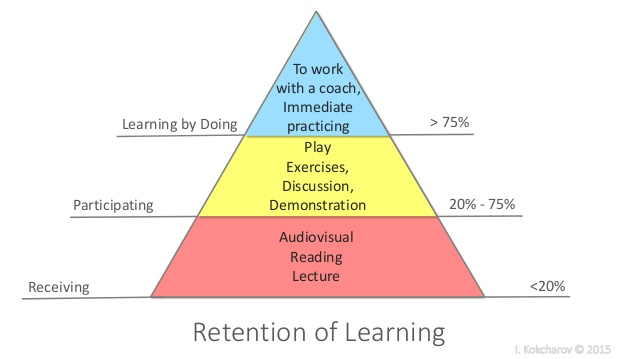
\includegraphics[width=0.8\linewidth]{figure/Analysis/skillslearn}
			\label{fig:ActiveLearn}
			\caption{Retention of Learning, taken from \href{https://www.slideshare.net/igorkokcharov/kokcharov-skillpyramid2015}{\color{blue}here}}
		\end{figure}
	\subsection*{Passive Learning}
	
	
	\subsection{Interactivity of music learning}	
When trying to understand music in an interactive sense, one might look at another medium that incorporates interactivity: video games. In particular, one could look at interactive video games that focuses on playing or teaching music. Lily Gower and Janet McDowall conducted a study, in 2012, centered around the educational qualities gained from playing such interactive music video games\cite{interactiveMusicVideoGames}. The study aimed to establish if interactive music video games had an educational value when integrated into the existing music education.\\

The different games mentioned in the study were Guitar hero (See \autoref{sec:guitarHero}), SingStar and Wii Music. What these games have in common is that they all use interactivity as a means to playing music, be it with a guitar shaped controller, a microphone or the Wii remote held like an instrument. These games try to emulate what it would \textit{feel like} to play a guitar, sing or play different instruments.\\

The study interviewed two music teachers of different musical abilities, and 9 music students aged 11-14 (5 male and 4 female) from different socio-economic situations. The student participants came into the study with different levels of musical experience. The interviews were semi-structured of nature to allow free flowing conversation. Interviews with the children participants revolved around their prior music backgrounds and past experiences with interactive music video games. The interviews with the teacher participants discussed their personal views and experiences with interactive music video games, like Guitar hero (\autoref{sec:guitarHero}), in relation to music education.\\

Teacher two said during the interview that:
\begin{quote}
	\textit{"...the whole debate about whether it’s music making, that’s a whole other debate, but whether it’s developing some across the board generic skills, I’d say yes."}\cite[p.~98]{interactiveMusicVideoGames}.\\
\end{quote}
Meaning a belief in interactive music video games giving the students some educational values in a more general music setting. In addition, when asked about coordination benefits, Teacher two said the following:
\begin{quote}
	\textit{"...To play at the higher levels of that game [Guitar Hero] requires very high level coordination skills and you’re coordinating visually with what you’re playing as an instrument. So it’s not so different I think physiologically from what a musician does anyway which is to respond to a conductor visually, respond to the music score visually, and then play accordingly to a set tempo, and timing is everything. So, the game is about scoring high scores all based on your capacity to play in time on the right note and what’s that sound like? Sounds like music playing to me."}\cite[p.~98]{interactiveMusicVideoGames}.\\
\end{quote}
Teacher two has a firm belief that Guitar hero specifically has a high coordination requirement, and thus to play at the higher difficulty levels of the game, you need good eye-hand coordination, which he thinks correlates in a physiological way directly to the way real music is played.\\

When the student participants where asked about their musical knowledge gained from playing interactive music video games, one girl said:
\begin{quote}
	\textit{"Yeah, so it’s like you find out about more songs that you don’t know about . . . there’s a lot of songs that you don’t know about and then you like listen to them and then you get into either like the artist or the type of songs or you just listen to that song and stuff and then you go looking on the net for other songs of that type and stuff, so it opens up a whole lot of stuff."}\cite[p.~100]{interactiveMusicVideoGames}.\\
\end{quote}	
The participant felt that she had gained music knowledge, and broadened her musical identity. The exposure to the new music, gave her an interest in new artists and genres she might not have known about.\\

The discussion about whether or not interactive music video games provide the children with a basic understanding of essential musical elements, is argued by Lily Gower and Janet McDowalls, to be that they at least learned about pitch and rhythm, while maybe not the rest of the five elements seen in \autoref{list:basicMusic}. Meaning the interactive music video games assisted the children in Lily Gower and Janet McDowall's study develop some basic music skills, that might correlate to real music making\cite[p.~99]{interactiveMusicVideoGames}, and potentially could assist other children in similar age groups.

\subsubsection*{Sub conclusion}
In conclusion, the children in the study\cite{interactiveMusicVideoGames} did seem to learn at least two basic musical elements from interactive music video games, being pitch and rhythm. In addition the children also felt they had gained musical knowledge from these games. Hence interactivity in musical education, it being from Guitar Hero, SingStar or another interactive music medium, seems to assist children in development of some aspects of musical abilities.

\section{Motivation theory}\todo{Maybe a section on motivation}

Video game design and education relating to motivation\cite{motivationGameDesign}.


\begin{itemize}
	\item[ ] \textbf{Intrinsic motivation} pushes us to act freely, on our own, for the sake of it.\\
	\item[ ] \textbf{Extrinsic motivation} pulls us to act due to factors that are external to the activity itself, like reward or threat.\\
	\item[] \textbf{Amotivation} denotes the absence of motivation.\\
\end{itemize}

\begin{quote}
	\textit{Other key factors in motivation theory that can be identified within good video games include curiosity and a sense of autonomy or control over the learning that is occurring}\cite[p.~92]{interactiveMusicVideoGames}.\\
\end{quote}
\subsection{The element of Surprise}
Studies have shown that surprise and novelty integrated into music instruction, can stimulate the brain and thereby heighten children's interest, make them curious and pay attention\cite{bagpipesSurprise}. Also it will motivate exploratory behavior which will lead to an enhancement in learning.\todo{Write more if this is relevant}


Furthermore, adding an element of mystery...\todo{Write more on this here}

\section{Target Group}

\begin{itemize}
	\item[-] Elementary school children (Grade 1,2,3,4,5,6)
	\item[-] Potentially the teachers as a sub target group?\todo{Maybe other way around?}
\end{itemize}





\section{State of the art}\label{sec:sota}
	
	\subsection{Guitar hero}\label{sec:guitarHero}
		\begin{figure}[H]
			\centering
			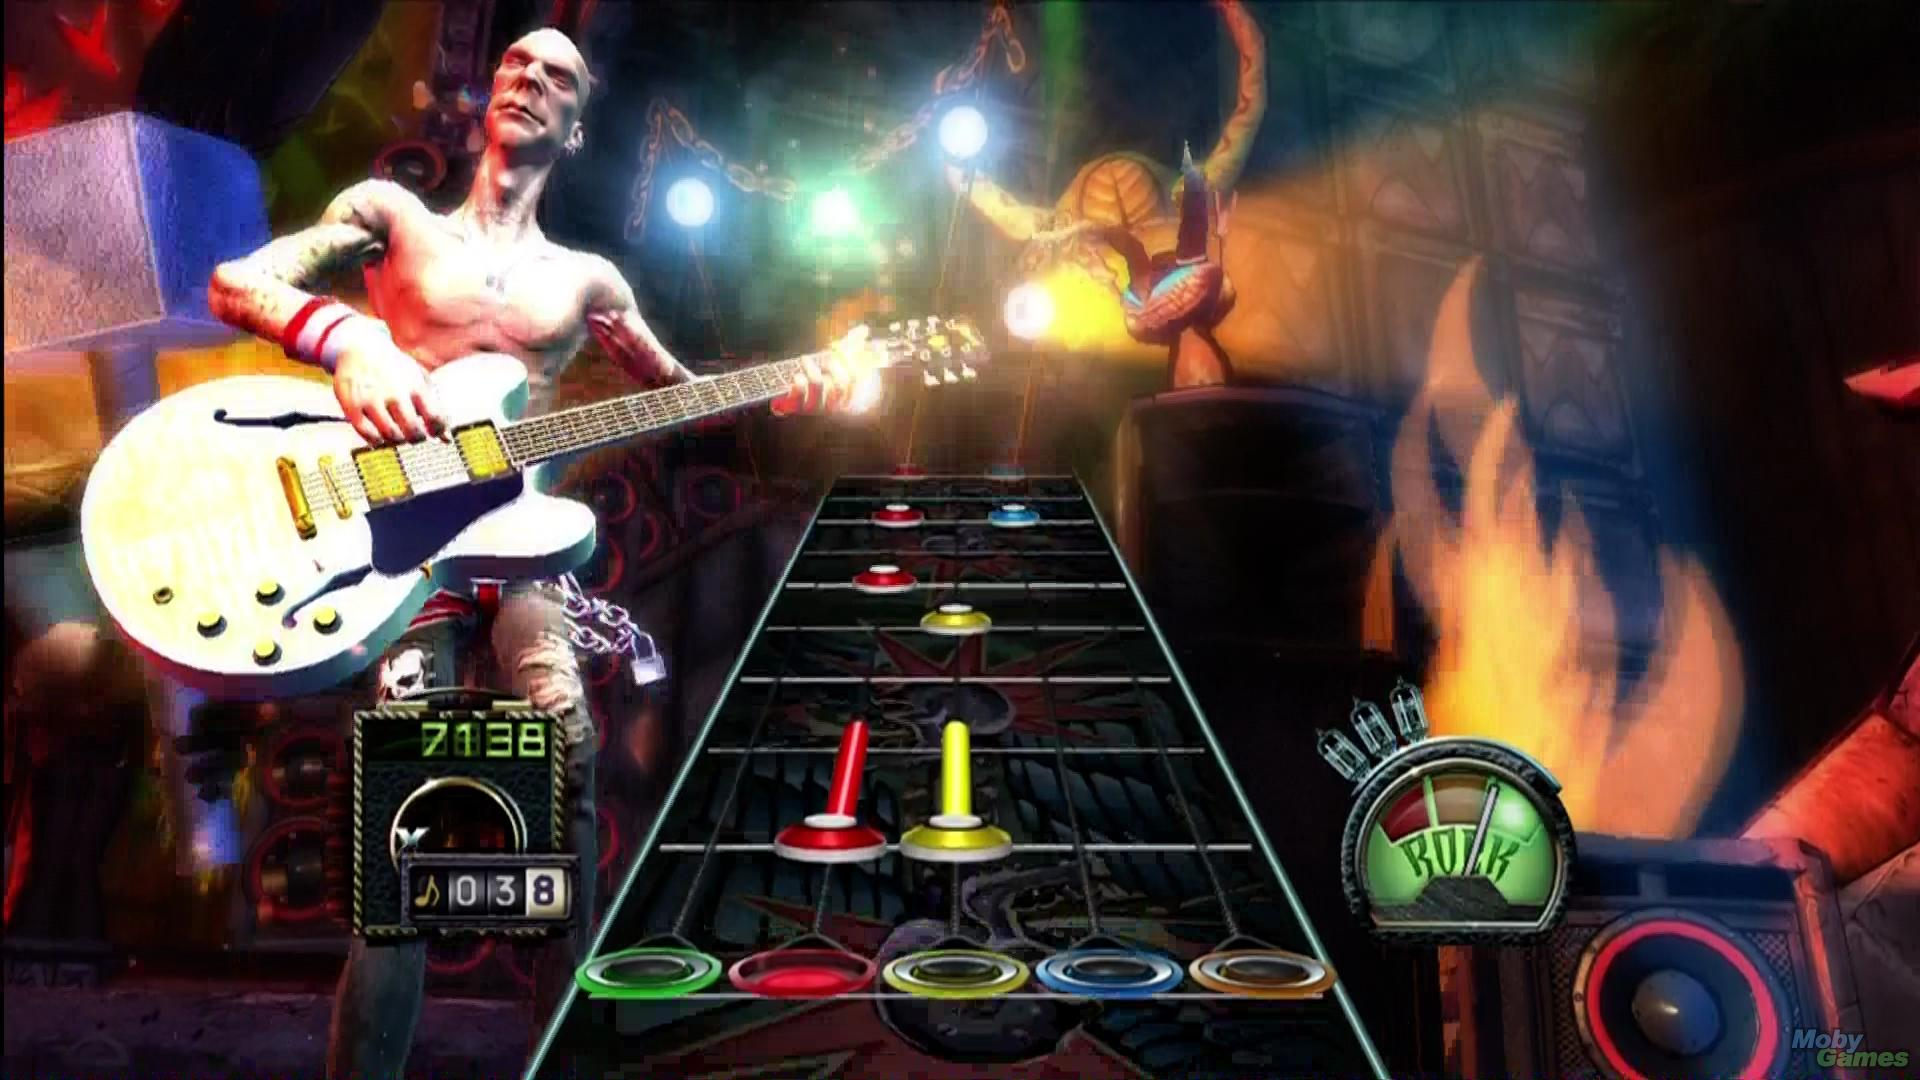
\includegraphics[width=0.7\linewidth]{figure/Analysis/guitarhero}
			\label{fig:guitarHero}
			\caption{Interactive music video game guitar hero.}
		\end{figure}
	\subsection{Noteput}
		German table where you physically put notes on it, and press play button to play notes, hopefully learning note and sheet theory.
	\subsection{Dato duo}
		Two person synthesizer for kids, no apparent learning outcome, but seems fun to play around with.
		\begin{figure}[H]
			\centering
			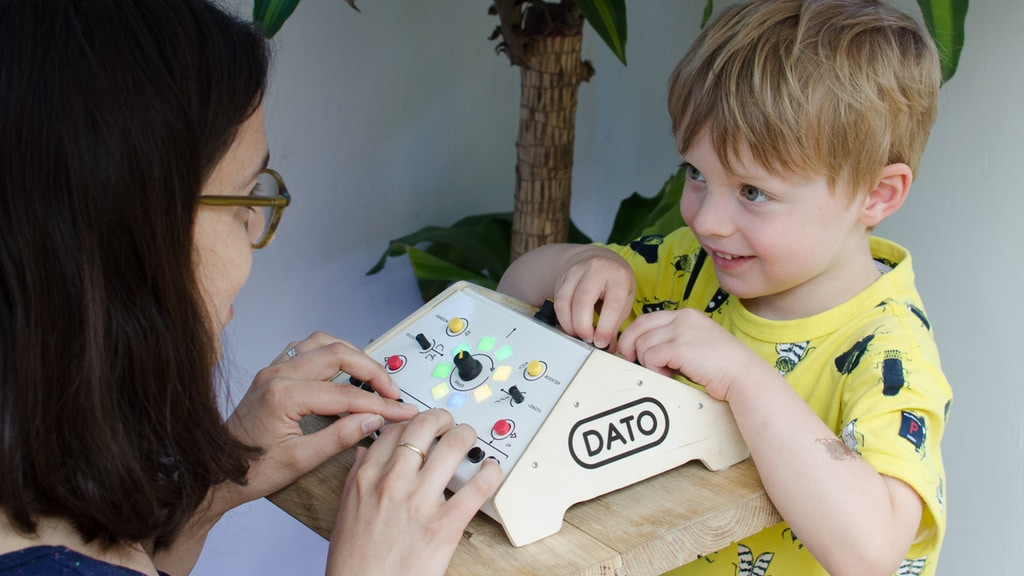
\includegraphics[width=0.7\linewidth]{figure/Analysis/datoduo}
			\label{fig:datoduo}
			\caption{Dato duo synthesizer}
		\end{figure}
	\subsection{Soundstage}
		VR application by Google, where you compose and play music in virtual reality. You can synthesize, plug things into other things, and create entire scores in this virtual reality playground.
		
	\subsection{V-Beat}
		The v-beat drumsticks are, for all its intents and purposes, simply air drumming.
		\begin{figure}[H]
			\centering
			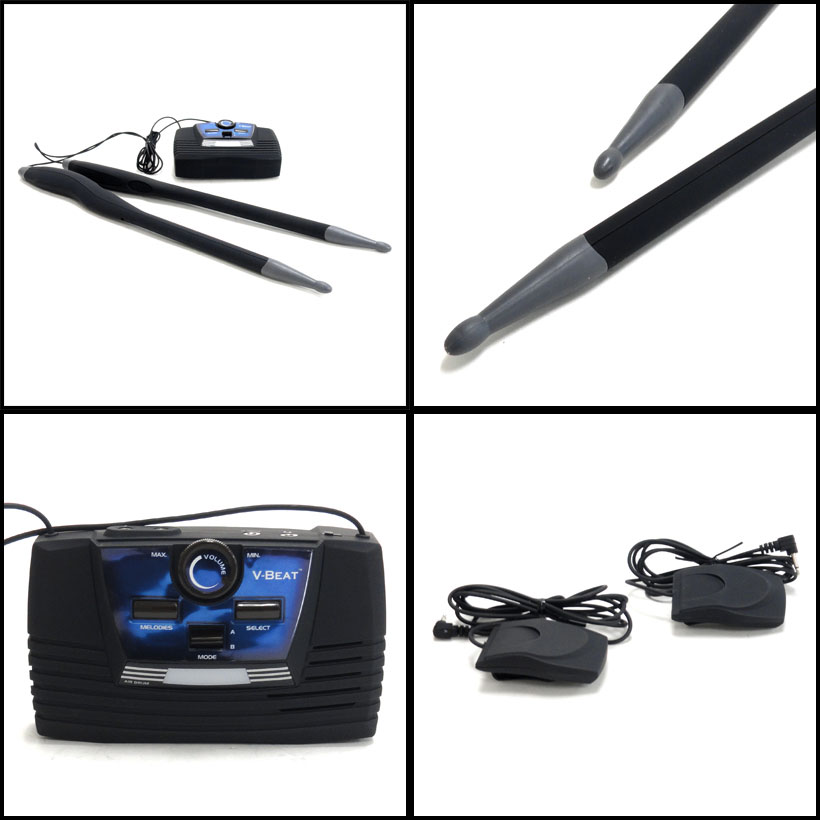
\includegraphics[width=0.5\linewidth]{figure/Analysis/vbeat}
			\label{fig:vbeat}
			\caption{Vbeat drumsticks}
		\end{figure}
		
	\subsection{MI Guitar}
		\begin{figure}[H]
			\centering
			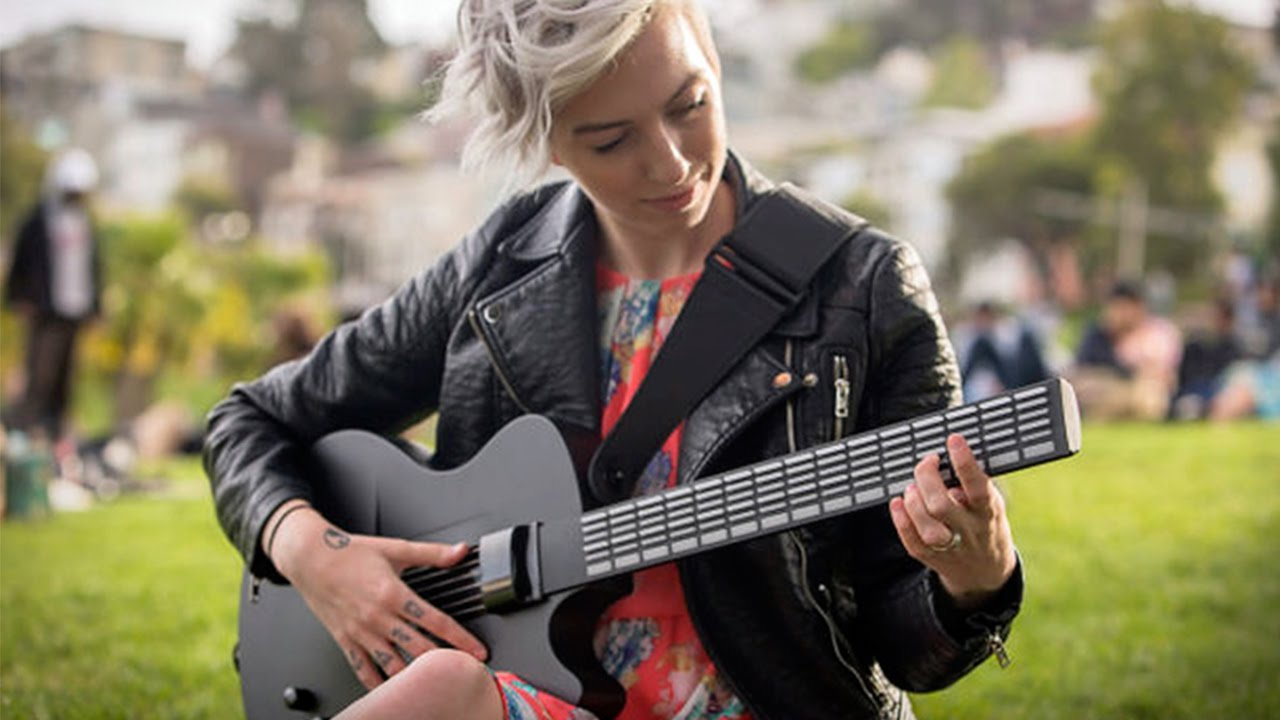
\includegraphics[width=0.8\linewidth]{figure/Analysis/miguitar}
			\label{fig:miguitar}
			\caption{MI guitar to teach guitar play}
		\end{figure}
	
	\subsection{Yousician}
		\begin{figure}[H]
			\centering
			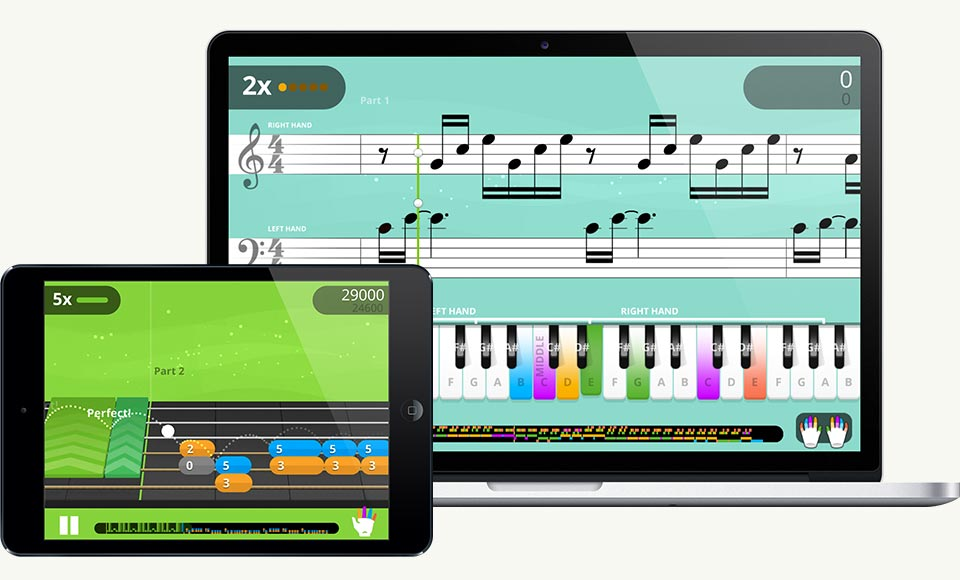
\includegraphics[width=0.8\linewidth]{figure/Analysis/yousician.jpg}
			\label{fig:yousician}
			\caption{Yousician}
		\end{figure}
	\subsection{Chrome Music Lab}
		\begin{figure}[H]
			\centering
			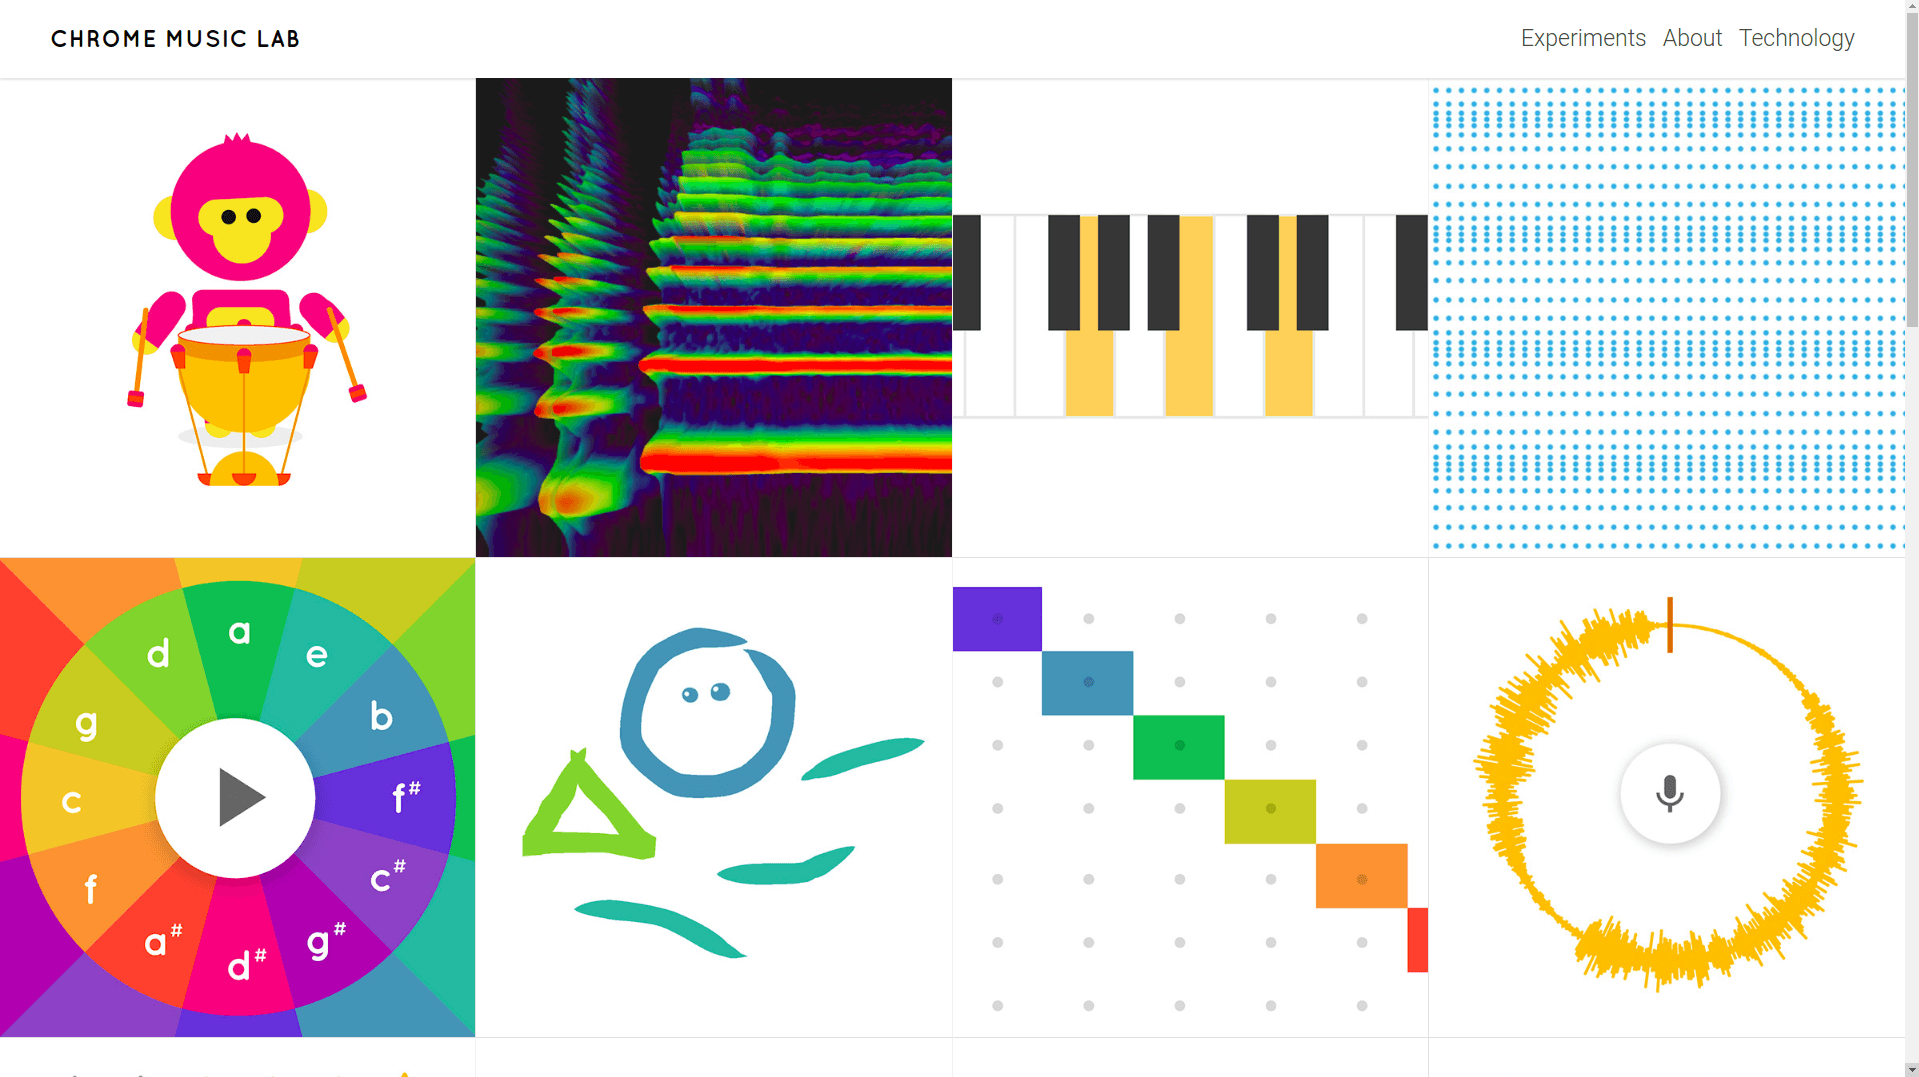
\includegraphics[width=0.8\linewidth]{figure/Analysis/chromeMusicLab.png}
			\label{fig:chromeMusicLab}
			\caption{Chrome Music Lab}
		\end{figure}

		